%============================================================
%  Защита ВКР — Дементьев С. А., каф. интеллектуального анализа данных, ФПМИ МФТИ, 2026
%  Компилятор: XeLaTeX (обязательно).  Рисунки — в папке pictures/.
%
%  Преамбула — из presentation_guide.md (тема/палитра/шрифты не изменены).
%  Добавлены только аддитивные строки, не меняющие тему/цвета/шрифт:
%    - tikz (схемы постановки и контура обратной связи),
%    - amssymb (порядок Лёвнера \succeq/\preceq),
%    - booktabs (таблицы с параметрами и соответствиями),
%    - frametitle size=\small (короткие описательные заголовки),
%    - скрыты навигационные символы.
%
%  На слайдах — только тезисы/формулы/рисунки; развёрнутая речь — в speech.md.
%============================================================
\documentclass[aspectratio=43]{beamer}
\usepackage[utf8]{inputenc}
\usepackage{xeCJK}
\usepackage{graphicx}
\usepackage{mathtools}
\usepackage{utopia}
\usetheme{CambridgeUS}
\usecolortheme{dolphin}

% Поддержка русского языка
\usepackage[utf8]{inputenc}
\usepackage[T2A, T1]{fontenc}
\usepackage{fontspec}
\usefonttheme{serif}
\setmainfont{Times New Roman}

% Цветовая схема (фиолетовая палитра)
\definecolor{myNewColorA}{RGB}{126,12,110}
\definecolor{myNewColorB}{RGB}{165,85,154}
\definecolor{myNewColorC}{RGB}{203,158,197}
\setbeamercolor*{palette primary}{bg=myNewColorC}
\setbeamercolor*{palette secondary}{bg=myNewColorB, fg=white}
\setbeamercolor*{palette tertiary}{bg=myNewColorA, fg=white}
\setbeamercolor*{titlelike}{fg=myNewColorA}
\setbeamercolor*{title}{bg=myNewColorA, fg=white}
\setbeamercolor*{item}{fg=myNewColorA}
\setbeamercolor*{caption name}{fg=myNewColorA}
\usefonttheme{professionalfonts}

\usepackage[numbers]{natbib}
\usepackage{hyperref}

% Размеры шрифтов на титульном слайде
\setbeamerfont{title}{size=\large}
\setbeamerfont{subtitle}{size=\small}
\setbeamerfont{author}{size=\small}
\setbeamerfont{date}{size=\small}
\setbeamerfont{institute}{size=\small}

%---- аддитивные строки (тему/палитру/шрифт не меняют) ----
\usepackage{amssymb}
\usepackage{booktabs}
\usepackage{tikz}
\usetikzlibrary{arrows.meta, positioning, calc}
\setbeamerfont{frametitle}{size=\small}
\setbeamertemplate{navigation symbols}{}
%----------------------------------------------------------

\title[Скрытые петли обратной связи в RecSys]{Алгоритм распознавания скрытых петель обратной связи\\ в рекомендательных системах}
\subtitle{Выпускная квалификационная работа бакалавра}
\author[Дементьев С.\,А.]{Дементьев Сергей Андреевич}
\institute[МФТИ]{Кафедра интеллектуального анализа данных, ФПМИ МФТИ\\
ВЦ им. А.\,А. Дородницына РАН\\
\vspace{0.4em}Научный руководитель: к.ф.-м.н. Хританков А.\,С.}
\date[2026]{Москва, 2026}

\begin{document}

%============================================================
% Слайд 1 — Титульный
%============================================================
\frame{\titlepage}

%============================================================
\section{Постановка}

% Слайд 2 — Постановка задачи (только тезисы)
\begin{frame}{Постановка задачи}
\footnotesize

\begin{columns}[T]
\column{0.5\textwidth}

\textcolor{myNewColorA}{\textbf{Объект:}} рекомендательная система, переобучаемая на данных, порожденных собой же.

\vspace{0.5em}
\textcolor{myNewColorA}{\textbf{Проблема.}} Система переобучается на собственных логах, а пользователь кликает по \emph{показанному}. Наблюдаемые метрики (CTR, NDCG) растут, но как оценки они смещены. Под воздействием рекомендательной системы аудитория изменяется.

\column{0.5\textwidth}
\textcolor{myNewColorA}{\textbf{Цель:}} построить модель эффекта как динамическую систему; установить условия деградации, \textbf{отделив вклад переобучения}.

\vspace{0.4em}
\textcolor{myNewColorA}{\textbf{Задачи:}}
\begin{enumerate}\setlength\itemsep{0.15em}
  \item формализовать петлю как динамическую систему;
  \item оценить скорость стягивания разнообразия;
  \item найти, где измерим след переобучения;
  \item проверить предсказания численно.
\end{enumerate}
\end{columns}

\vspace{0.7em}

\end{frame}

%============================================================
% Слайд 3 — Общая постановка RecSys
\begin{frame}{Данные рекомендательной системы — пары пользователь--объект}
\footnotesize

\begin{columns}[T]
\column{0.43\textwidth}
\begin{center}
\begin{tikzpicture}[
  >={Stealth[length=2mm]}, node distance=9mm,
  user/.style={draw=myNewColorA, very thick, circle, fill=myNewColorC!35,
               minimum size=8mm, inner sep=1pt, font=\scriptsize},
  item/.style={draw=myNewColorA, very thick, rounded corners, fill=myNewColorC!35,
               minimum width=11mm, minimum height=7mm, inner sep=2pt, font=\scriptsize},
  edge/.style={->, thick, myNewColorA}]
  \node[user] (u1) {$u_1$};
  \node[user, below=of u1] (ui) {$u_i$};
  \node[user, below=of ui] (un) {$u_N$};
  \node[item, right=25mm of u1] (v1) {$v_1$};
  \node[item, below=of v1] (vj) {$v_j$};
  \node[item, below=of vj] (vm) {$v_M$};
  \draw[edge] (u1)--(v1);
  \draw[edge] (ui)--node[above, font=\tiny]{$Y_{ij}=1$}(vj);
  \draw[edge] (ui)--(v1);
  \draw[edge] (un)--(vm);
  \node[font=\scriptsize, text=myNewColorA] at ($(u1)!0.5!(v1)+(0,0.7)$) {наблюдаемые взаимодействия};
\end{tikzpicture}
\end{center}

\column{0.57\textwidth}
\textcolor{myNewColorA}{\textbf{Объекты постановки.}}
\begin{itemize}\setlength\itemsep{0.25em}
  \item пользователи $u_i$, объекты каталога $v_j$;
  \item датасет:
  \[
    \mathcal B=\{(u_i,v_j,y_{ij}):(i,j)\in\Omega\};
  \]
  \item $y_{ij}$ — зафиксированный отклик: покупка, клик, положительная оценка.
  \item $u, v \in \mathbb{R}^n$. Вложение построено так, что $\langle u, v\rangle$ является мерой релевантности объекта $v$ для пользователя $u$.
\end{itemize}

\vspace{0.2em}
В рек. системах используют регрессию, обучение метрике и ранжирование; в этой работе — \textbf{предсказание клика}.
\end{columns}

\vspace{0.6em}
\begin{center}
\[
Y_{ij}\sim\operatorname{Bern}\!\bigl(\eta(u_i,v_j)\bigr),\qquad
\eta(u_i,v_j)=\mathbb P(Y_{ij}=1\mid u_i,v_j).
\]
\end{center}
\end{frame}

%============================================================
% Слайд 4 — Контур как система управления
\begin{frame}{Динамическая система для средних}
\scriptsize
\begin{center}
\begin{tikzpicture}[
  >={Stealth[length=2mm]}, node distance=9mm,
  box/.style={draw=myNewColorA, very thick, rounded corners, fill=myNewColorC!40,
              align=center, minimum height=8mm, inner sep=3pt, font=\scriptsize},
  arr/.style={->, very thick, myNewColorA}]
  \node[box] (r) {Модель $f_t$};
  \node[box, right=of r] (s) {Выдача\\ top-$L$};
  \node[box, right=of s] (c) {Клики\\ пользователя};
  \node[box, right=of c] (l) {Логи};
  \draw[arr] (r)--(s); \draw[arr] (s)--(c); \draw[arr] (c)--(l);
  \draw[arr] (l.north) .. controls +(0,0.9) and +(0,0.9) ..
       node[above, font=\scriptsize, text=myNewColorA]{переобучение модели} (r.north);
\end{tikzpicture}
\end{center}

\vspace{-0.1em}
\begin{columns}[T]
\column{0.5\textwidth}
\begin{equation*}
\begin{aligned}
\theta_t^{ij}:=\theta(u_i^t,v_j)
&=\sigma\!\left(\frac{\langle u_i^t,v_j\rangle}{\tau}\right),\\
\sigma(z)&=\frac{1}{1+e^{-z}}
\end{aligned}
\tag{1}
\end{equation*}
\begin{equation*}
f_t^{ij}:=f(u_i^t,v_j;w^t)\in[0,1]
\tag{2}
\end{equation*}
\begin{equation*}
S_i^t=\operatorname{TopL}_{j\in\mathcal I_i^t} f_t^{ij},\qquad |S_i^t|=L
\tag{3}
\end{equation*}

\column{0.5\textwidth}
\begin{equation*}
\eta_t^{ij}=(1-\alpha)\theta_t^{ij}+\alpha f_t^{ij},\qquad
\alpha=\rho s\in[0,1]
\tag{4}
\end{equation*}
\begin{equation*}
Y_t^{ij}\sim\operatorname{Bern}(\eta_t^{ij}),\qquad j\in S_i^t
\tag{5}
\end{equation*}

\begin{equation*}
\begin{aligned}
u_i^{t+1}
&=(1-\rho)u_i^t+\rho\bigl((1-\beta)u_i^t+\beta v_{j_i^t}\bigr),\\
\mathbb P(a_i^t=1)&=\rho,\qquad \beta\in[0,1].
\end{aligned}
\tag{6}
\end{equation*}

\end{columns}

\vspace{0.2em}
\begin{center}
\textcolor{myNewColorA}{\textbf{Система в замкнутом виде:}}
$z_t=(x_t,w^t,\mathcal B_t)$, \quad
$z_{t+1}=\Phi_t(z_t,\xi_t)$.

{\scriptsize Выдача выбирается как управляющее воздействие.}
\end{center}
\end{frame}

%============================================================
% Слайд 5 — Задача стабилизации дискретного управления
\begin{frame}{Оптимальное управление максимизирует качество при стабилизации аудитории}
\footnotesize
\setlength{\abovedisplayskip}{0.35em}
\setlength{\belowdisplayskip}{0.35em}
\setlength{\abovedisplayshortskip}{0.2em}
\setlength{\belowdisplayshortskip}{0.2em}

\begin{columns}[T,onlytextwidth]
\column{0.48\textwidth}
\textcolor{myNewColorA}{\textbf{Дискретная управляемая система}}
\[
\begin{aligned}
a_t=\Pi_t(z_t)\in\mathcal A(z_t),
\qquad
z_{t+1}&=\Phi_t(z_t,a_t,\xi_t).
\end{aligned}
\]
{\scriptsize $a_t$ — выбранная выдача; $\Pi_t$ — политика управления.}

\vspace{0.15em}
\textcolor{myNewColorA}{\textbf{Стабилизируемая величина}}
\[
D_k^t=\operatorname{tr}\Sigma_k^t,\qquad
D^t=\sum_{k=1}^{K}\pi_kD_k^t.
\]
{\scriptsize $\Sigma_k^t$ — ковариация пользователей сегмента $k$; $D_k^t$ не оптимизируется, а удерживается в допустимой зоне.}

\column{0.48\textwidth}
\textcolor{myNewColorA}{\textbf{Функционал качества рекомендаций}}
\[
Q(t)=\mathbb E_{(i,j)\sim\mu_t}\,\mathbb E_y\,g(y),
\qquad 0\le g\le L.
\]
{\scriptsize $\mu_t$ — распределение показанных пар; $g$ — ограниченная функция отклика.}

\vspace{0.15em}
\[
\begin{aligned}
Q^{\mathrm{obs}}(t)&:\quad y\sim\mathrm{Bern}(\eta_t^{ij}),\\
Q^{\mathrm{true}}(t)&:\quad y\sim\mathrm{Bern}(\theta_t^{ij}).
\end{aligned}
\]
\end{columns}

\vspace{0.15em}
\textcolor{myNewColorA}{\textbf{Задача стабилизации дискретного управления}}
{\tiny
\[
\begin{aligned}
\boldsymbol\Pi^\star\in
\arg\max_{\boldsymbol\Pi\in\mathfrak P}\quad
&\mathbb E_{\boldsymbol\Pi}\!\left[
\frac1T\sum_{t=0}^{T-1}Q^{\mathrm{true}}(t)\right] \\
\text{при}\quad
&a_t=\Pi_t(z_t),\qquad
z_{t+1}=\Phi_t(z_t,a_t,\xi_t),\\
&\underline D_k\le
\mathbb E_{\boldsymbol\Pi}D_k^t
\le \overline D_k,\\
&k=1,\ldots,K,\qquad t=1,\ldots,T .
\end{aligned}
\]
Для каждого сегмента задаётся допустимый коридор разнообразия.}
\end{frame}

%============================================================
% Слайд 6 — Завышение наблюдаемых метрик
\begin{frame}{Расхождение между наблюдаемым и истинным качеством}
\footnotesize

\begin{columns}[T]
\column{0.48\textwidth}
\textcolor{myNewColorA}{\textbf{Предложение 3.1: самоподкрепление}}
\[
\Delta_{\eta,t}
=(1-\alpha)\Delta_{\theta,t}+\alpha\Delta_{f,t}.
\]
{\scriptsize $\Delta_{\theta,t}$, $\Delta_{f,t}$, $\Delta_{\eta,t}$ — истинная, модельная и наблюдаемая разности отклика для двух объектов.}

\vspace{0.6em}
Если модель поставила $j$ выше $j'$, но истинный порядок противоположен:
\[
\Delta_{f,t}>0,\qquad \Delta_{\theta,t}=-D<0,
\]
то логи всё равно подтвердят модель при
\[
\alpha>\frac{D}{D+\Delta_{f,t}}.
\]

\column{0.52\textwidth}
\textcolor{myNewColorA}{\textbf{Предложение 3.2: канал разрыва качества}}
\[
\begin{aligned}
\bigl|Q^{\mathrm{obs}}(t)-Q^{\mathrm{true}}(t)\bigr|
&\le L\,\mathbb E_{\mu_t}\!\left|\eta_t^{ij}-\theta_t^{ij}\right|\\
&\le L\sqrt{\frac12\,\overline{\mathrm{KL}}_t}.
\end{aligned}
\]
\[
\overline{\mathrm{KL}}_t=
\mathbb E_{\mu_t}\,
\mathrm{KL}\!\left(
\mathrm{Bern}(\eta_t^{ij})\,\Vert\,
\mathrm{Bern}(\theta_t^{ij})\right).
\]
{\scriptsize Второе неравенство — следствие неравенства Пинскера и вогнутости корня.}
\end{columns}

\vspace{0.65em}

\end{frame}

\section{Теоретические результаты}

%============================================================
% Слайд 7 — Теорема 1: оценка стягивания разнообразия
\begin{frame}{Теоретические оценки вырождения аудитории}
\footnotesize

\large{\textcolor{myNewColorA}{\textbf{Теорема 1} (Дементьев, 2026)}}\normalsize
\vspace{0.25em}

{\footnotesize Пусть:}



\[
D_k^t=\operatorname{tr}\Sigma_k^t,\qquad
M_k^t:=\frac1{n_k}\sum_{i\in\mathcal C_k}\|u_i^t-\bar v_k\|^2,\qquad
D_k^t\le M_k^t.
\]
{\footnotesize И при условиях (A1) - (A4):}

\vspace{0.2em}
\[
\boxed{\;
\mathbb E D_k^t
\le
M_k^0q^t+\frac{\beta\sigma_\xi^2}{2-\beta},
\qquad
q=1-\beta\rho(2-\beta)<1.
\;}
\]
\end{frame}

%============================================================
% Слайд 8 — Гауссова модель рекомендаций
\begin{frame}{Частный случай модели гауссовой смеси}
\footnotesize

\begin{columns}[T]
\column{0.55\textwidth}
\textcolor{myNewColorA}{\textbf{Фиксируем кластер вкусов $k$.}}
{\scriptsize $v\in\mathbb R^d$ — вектор объекта; $\mu_k$ — центр тематики; $\Psi_k$ — естественный разброс каталога.}
\[
V_k^{\mathrm{cat}}\sim\mathcal N(\mu_k,\Psi_k).
\]

\vspace{-0.2em}
\textcolor{myNewColorA}{\textbf{Рекомендатель заостряет каталог.}}
\[
r_k^t(v)=
-\frac12\,(v-\mu_k)^\top A_k^t(v-\mu_k),
\qquad A_k^t\succeq0.
\]
{\scriptsize $A_k^t$ — \textbf{резкость} выдачи: чем больше $A$, тем сильнее штраф за удаление от центра.}

\[
\pi_k^t(\mathrm dv)\propto
\exp\{r_k^t(v)\}\,
\mathcal N(\mu_k,\Psi_k)(\mathrm dv).
\]
\[
V_k^t\sim\mathcal N(\mu_k,C_k^t),
\qquad
\boxed{\;C_k^t=(\Psi_k^{-1}+A_k^t)^{-1}\;}
\]

\column{0.45\textwidth}
\begin{center}
\begin{tikzpicture}[scale=0.82]
  \draw[->, myNewColorA, thick] (-2.35,0) -- (2.45,0) node[right, font=\scriptsize] {$v_1$};
  \draw[->, myNewColorA, thick] (0,-1.65) -- (0,1.75) node[above, font=\scriptsize] {$v_2$};

  \draw[myNewColorB, very thick, dashed, fill=myNewColorC!18]
    (0,0) ellipse (1.95 and 1.15);
  \draw[myNewColorA, very thick, fill=myNewColorA!14]
    (0,0) ellipse (1.05 and 0.55);
  \fill[myNewColorA] (0,0) circle (2pt)
    node[below right, font=\scriptsize] {$\mu_k$};

  \node[align=center, font=\scriptsize, text=myNewColorB] at (-1.45,1.38)
    {каталог\\$\Psi_k$};
  \node[align=center, font=\scriptsize, text=myNewColorA] at (1.35,0.85)
    {выдача\\$C_k^t$};

  \draw[->, very thick, myNewColorA] (-1.65,-1.28) -- (-0.78,-0.62);
  \node[align=center, font=\scriptsize, text=myNewColorA] at (0.55,-1.35)
    {$A_k^t\uparrow$\\[-0.1em]$\Rightarrow C_k^t\downarrow$};
\end{tikzpicture}
\end{center}

\vspace{0.2em}
\textcolor{myNewColorA}{\textbf{Модельное упрощение.}}
{\scriptsize Политика $\pi_k^t$ общая для кластера: внутри сегмента модель не различает отдельных пользователей. Поэтому теорема говорит о кластерном механизме, а не о полной персонализации MLP.}
\end{columns}

\vspace{0.5em}

\end{frame}


%============================================================
\section{Эксперименты}

% Слайд 10 — Постановка вычислительного эксперимента
\begin{frame}{Описание эксперимента}
\footnotesize
\textbf{Шаг симуляции:} top-$L$ $\rightarrow$ клики $\rightarrow$ логи $\rightarrow$ $\beta$-дрейф $\rightarrow$ переобучение $\rightarrow$ метрики.

\vspace{0.8em}
\textcolor{myNewColorA}{\textbf{Четыре режима} — чтобы разделить эффекты взаимодействия}
\begin{itemize}\setlength\itemsep{0.2em}
\item \texttt{closed\_loop} — полная петля;
\item \texttt{static} — модель заморожена, $\alpha>0$ (без переобучения);
\item \texttt{fresh\_oracle} — честное переобучение;
\item \texttt{no\_influence} — $\alpha=0$.
\end{itemize}
\texttt{closed\_loop} $-$ \texttt{static} $=$ вклад переобучения.

\vspace{0.8em}
\textbf{Данные:} синтетические данные (GMM) и MovieLens-20M.
\end{frame}

%============================================================
% Слайд 11 — Совместный результат: beta-sweep и KL-grid для прогретых моделей
\begin{frame}{$\beta$-дрейф и петлевой KL-сигнал разделяются}
\scriptsize
\vspace{-0.3em}

\begin{center}
\textcolor{myNewColorA}{\textbf{Влияние $\beta$:}} при $\beta=0$ коллапса нет; при $\beta>0$ объём стягивается во всех режимах с $\alpha>0$.
\end{center}

\vspace{-0.75em}
\begin{center}
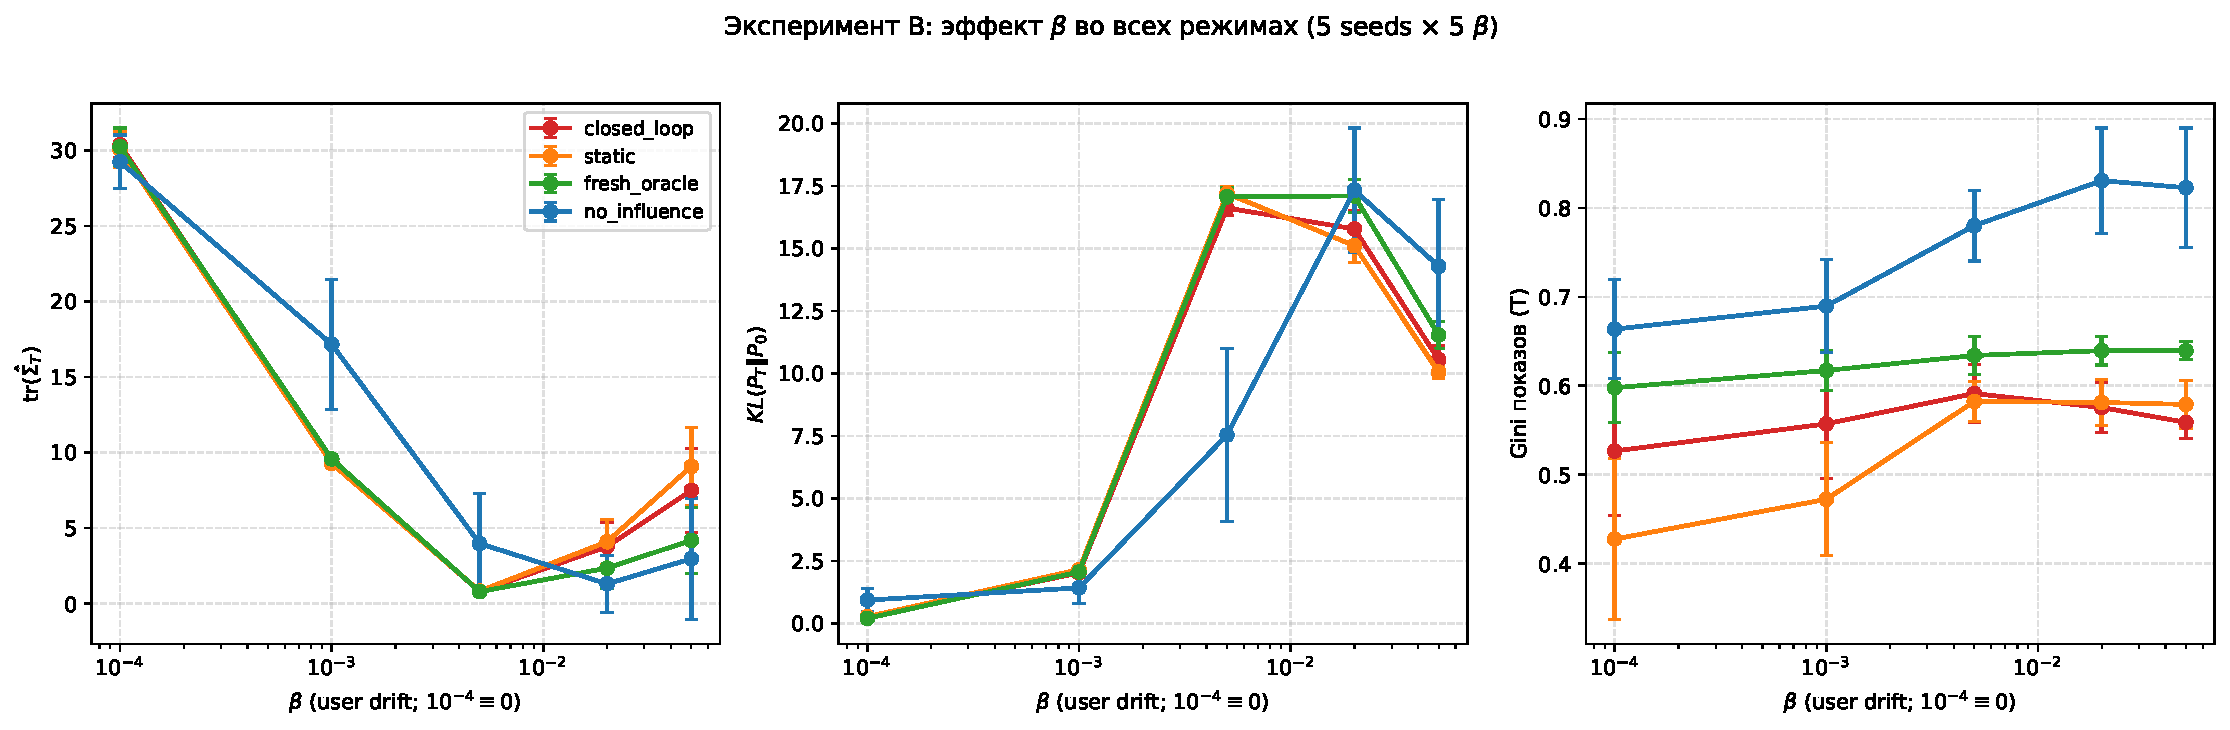
\includegraphics[width=0.95\linewidth,height=0.28\textheight,keepaspectratio]{pictures/beta_sweep.pdf}
\end{center}

\vspace{-0.75em}
\begin{center}
\textcolor{myNewColorA}{\textbf{Анализ KL-дивергенции:}} оставлены предобученные \texttt{warm} и \texttt{warm\_noisy}; петлевой вклад виден как разрыв \texttt{closed\_loop}$-$\texttt{static}.
\end{center}

\vspace{-0.75em}
\begin{center}
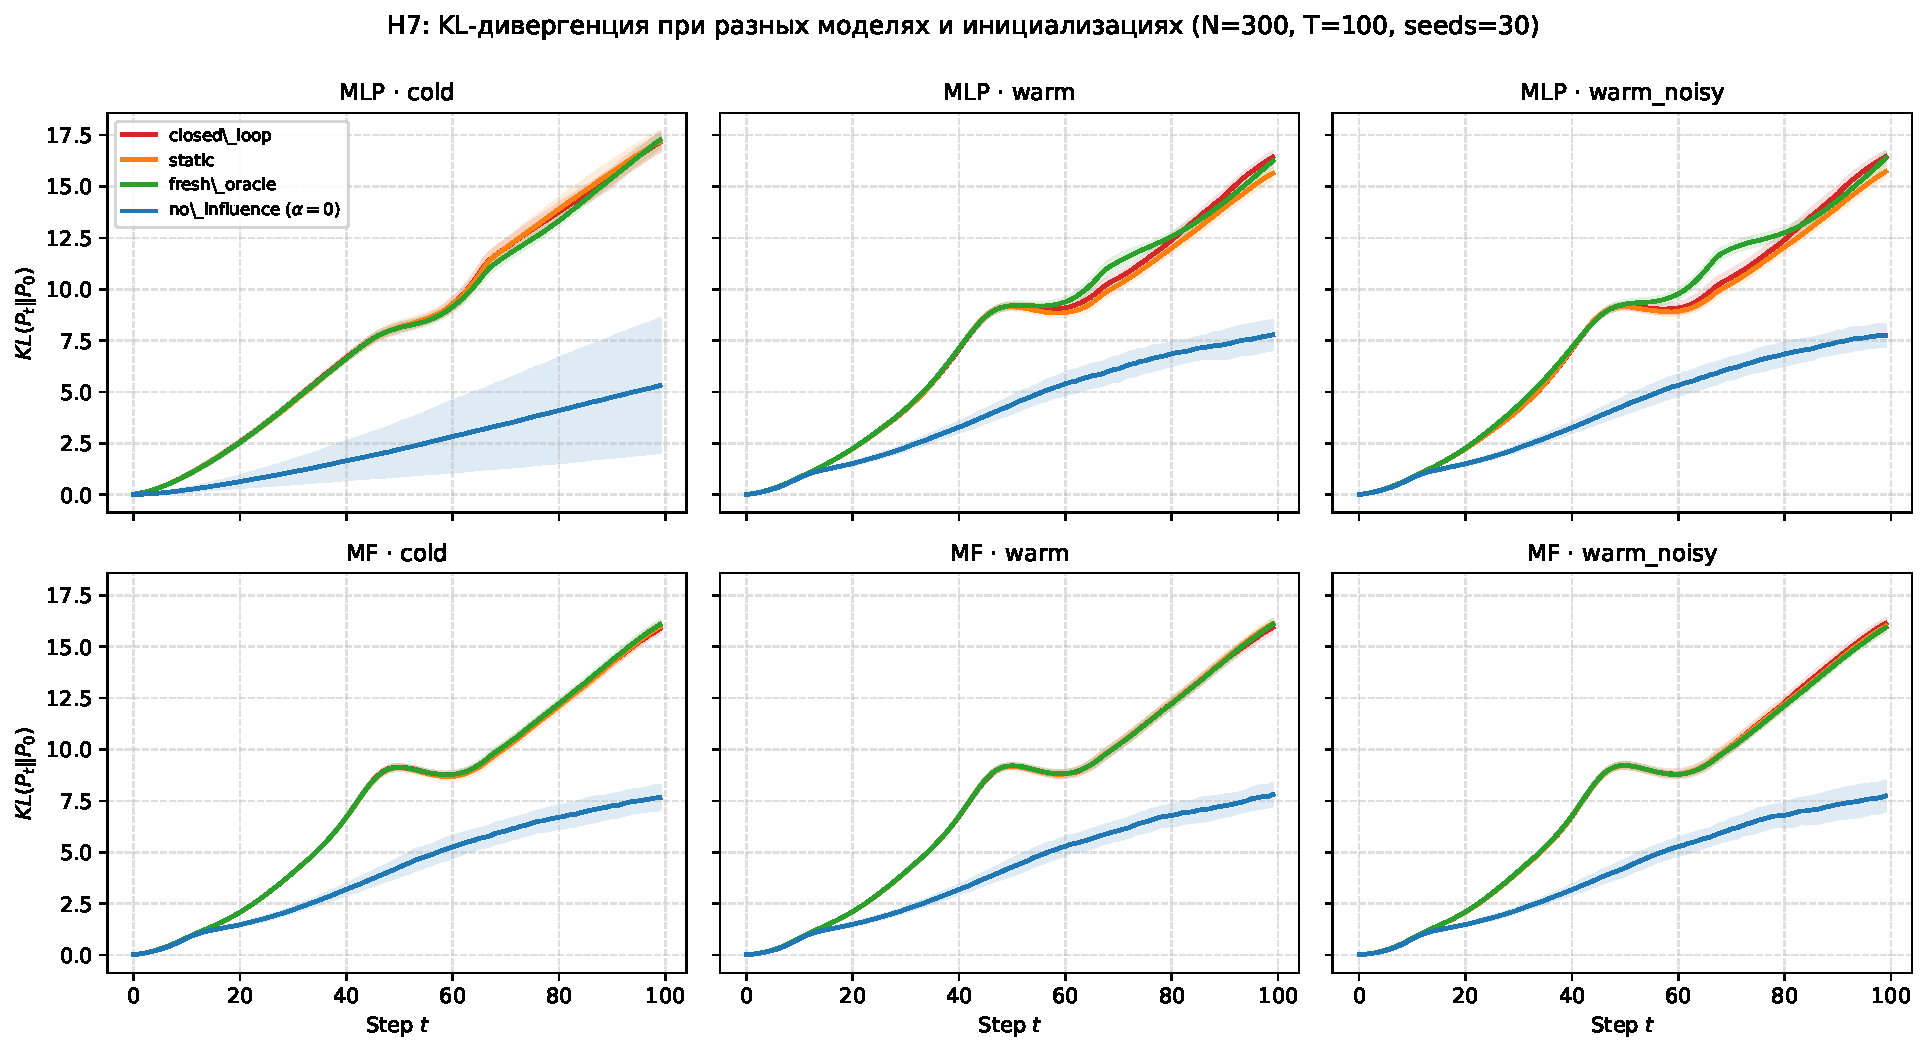
\includegraphics[
  width=0.98\linewidth,
  height=0.41\textheight,
  trim=0 0 0 30,
  clip,
  keepaspectratio
]{pictures/kl_grid.pdf}
\end{center}
\end{frame}

%============================================================
% Слайд 12 — Результат 2: воспроизводимость на MovieLens-20M
\begin{frame}{Воспроизводимость на MovieLens-20M}
\footnotesize
\begin{center}\scriptsize
Слева — коллапс разнообразия $\operatorname{tr}\hat\Sigma_u^t$; справа — дрейф распределения вкусов $\mathrm{KL}(P^t\Vert P^0)$.
\end{center}

\begin{figure}
\centering
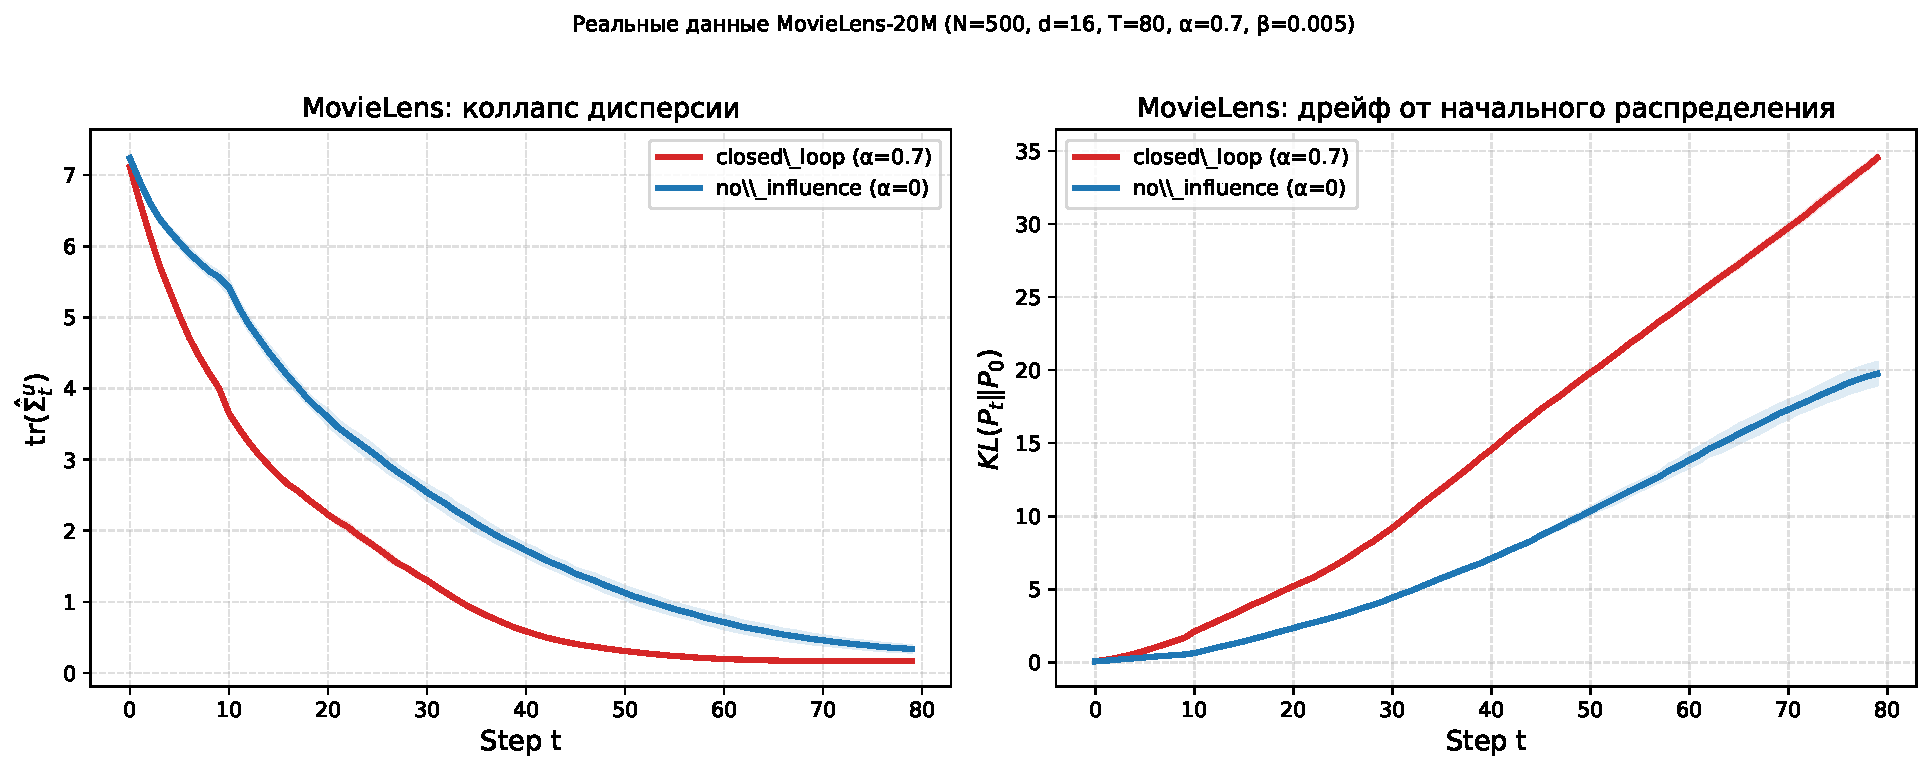
\includegraphics[width=0.86\linewidth,height=0.62\textheight,keepaspectratio]{pictures/movielens.pdf}
\end{figure}

\begin{center}
\textcolor{myNewColorA}{\textbf{Вывод.}} Система с петлёй обратной связи будет иметь $tr \Sigma^t_k$ и $KL$ отличающимися от режима без петли. Эти функционалы позволяют хорошо диагностировать петлю на реальных данных
\end{center}
\end{frame}

%============================================================
% Слайд 13 — Результат 1: универсальный коллапс объёма
\begin{frame}{Коллапс популяции — это следствие дрейфа (6), а не петли (4)}
\footnotesize
\begin{center}\scriptsize
Слева — разнообразие $\operatorname{tr}\hat\Sigma^t$ по четырём режимам; справа — фазовая диаграмма по загрязнению $\alpha$ и активности $\rho$.
\end{center}

\begin{figure}
\centering
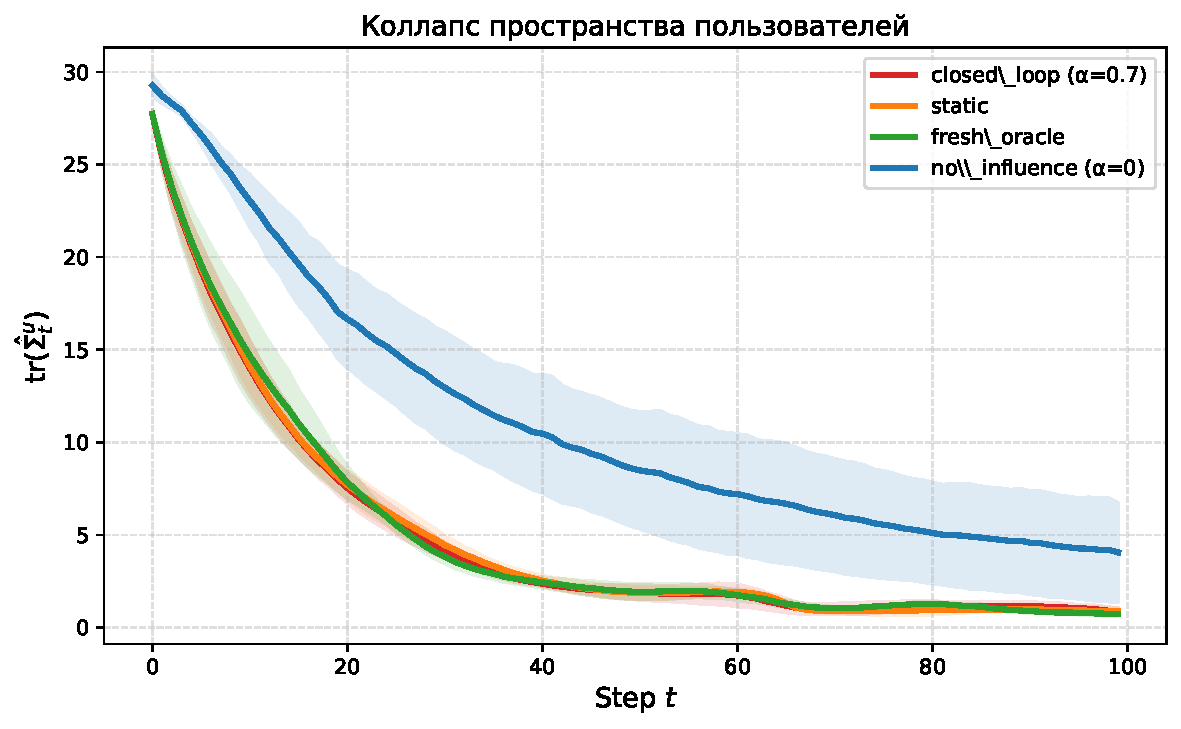
\includegraphics[width=0.50\linewidth,height=0.58\textheight,keepaspectratio]{pictures/trace_sigma_regimes.pdf}\hfill
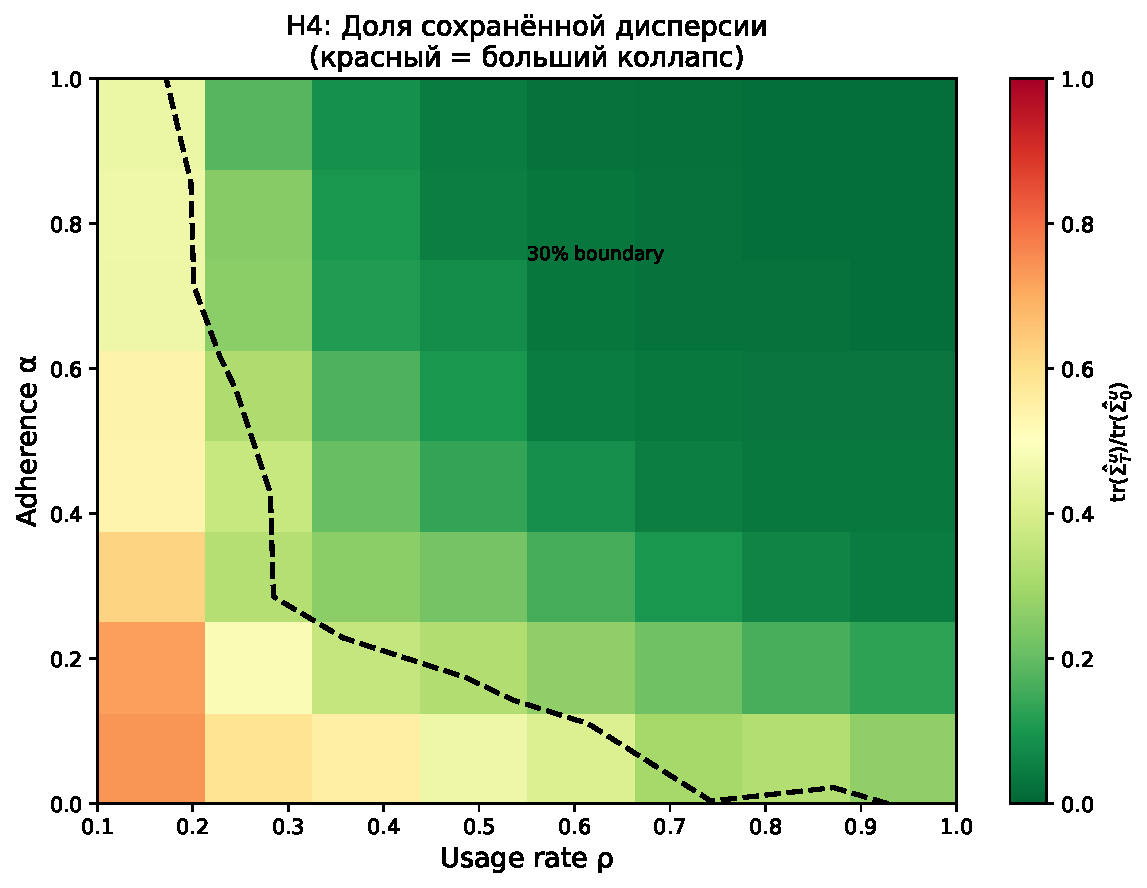
\includegraphics[width=0.44\linewidth,height=0.58\textheight,keepaspectratio]{pictures/phase_diagram.pdf}
\end{figure}

\begin{center}
\textcolor{myNewColorA}{\textbf{Вывод.}} Петля, заморозка и честное переобучение коллапсируют одинаково $\Rightarrow$ коллапс — это дрейф. \textbf{Теорема 1 подтверждена.}
\end{center}
\end{frame}

%============================================================
\section{Итоги}

% Слайд 14 — Выносится на защиту
\begin{frame}{Выносится на защиту}
\footnotesize

\begin{enumerate}\setlength\itemsep{0.6em}
\item \textcolor{myNewColorA}{\textbf{Математическая модель}} рекомендательной системы со скрытой петлей (динамическая система (1)-(6); предложения 3.1 и 3.2).
\item \textcolor{myNewColorA}{\textbf{Теорема 1 (Дементьев, 2026)}} о стягивании разнообразия; А также Теорема 2 (Дементьев, 2026) о переформировании выдачи.
\item \textcolor{myNewColorA}{Созданна имитационная модель}. Для неё был сделан экспериментальный стенд, который позволил проверить качественно свойства исследуемой системы
\item \textcolor{myNewColorA}{Получены парето-оптимальные политики} для экспериментального датасета MovieLens-20M, которые показывают качество лучше.
\end{enumerate}

\vspace{0.7em}
\begin{center}
\textcolor{myNewColorA}{Одобрение научным сообществом} Данное исследование выиграло 68-ую конференцию МФТИ. Работа подана на конференцию ICOMP.
\end{center}
\end{frame}

%============================================================
% Слайд 15 — Ограничения и дальнейшая работа
\begin{frame}{Ограничения и дальнейшая работа}
\scriptsize
\begin{columns}[T]
\column{0.5\textwidth}
\textcolor{myNewColorA}{\textbf{Ограничения}}
\begin{itemize}\setlength\itemsep{0.3em}
\item знак вклада петли в \emph{истинное} качество не установлен;
\item оценки некоторых эффектов имеют только качественный характер;
\item эксперименты проверяли практическую модель, а не теоретическую  
\end{itemize}

\column{0.5\textwidth}
\textcolor{myNewColorA}{\textbf{Дальнейшая работа}}
\begin{itemize}\setlength\itemsep{0.3em}
\item резкость $A$ и $\lVert J_k\rVert$ из весов как метрика риска;
\item раздельный анализ usage $p$ и adherence $s$;
\item решение задачи оптимального управления;
\item открытый приток пользователей.
\end{itemize}
\end{columns}
\end{frame}

%============================================================
\section{Источники}
% Слайд 16 — Список литературы
\begin{frame}{Список литературы}
\tiny
\nocite{*}
\bibliographystyle{plain}
\bibliography{refs}
\end{frame}

\end{document}
